\subsection{Locking}

\subsubsection{obterLockEscrita(TID, UID)}

\begin{figure}[H]
\centering
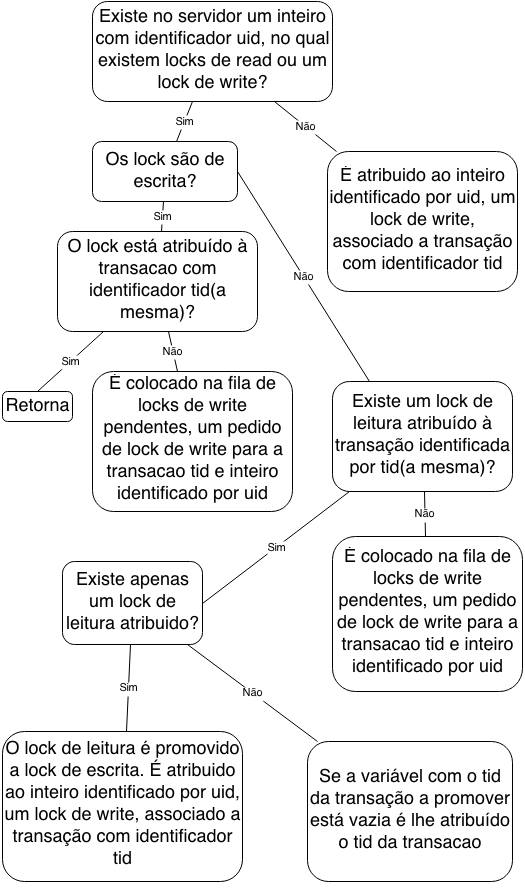
\includegraphics[width=8.25cm]{obtem_lock_w.jpg}
\caption{Obtenção de locks de escrita}
\end{figure}

\subsubsection{obterLockLeitura(TID, UID)}

Caso não exista no servidor um \textit{lock} de leitura ou escrita sobre o \textit{PadInt} identificado pelo \textit{UID} atribuído à transacção com \textit{TID}, é verificado se existe um \textit{lock} de escrita. Se existir é colocado na variável \textit{Leitores à espera} desse PadInt o \textit{TID}. Caso contrário é atribuído à transacção um \textit{lock} de leitura do \textit{PadInt}.

\subsubsection{libertarLockEscrita(TID, UID)}

O servidor remove o \textit{lock} de escrita da transacção identificada por \textit{TID}, associado ao inteiro identificado por \textit{UID}.

É invocado o método \textit{tiraQueueEscrita(UID)}, para que outras transações possam associar os seus locks ao mesmo PadInt.

\subsubsection{tiraQueueEscrita(UID)}

Se no \textit{PadInt} identificado pelo \textit{UID}, existir na variável \textit{Promoção} uma transacção a promover, essa transacção é removida da fila e é invocado o método \textit{obterLockEscrita(TID,UID)}. Caso contrário, é verificado se existe na fila de \textit{locks} de escrita pendentes do \textit{UID} alguma transacção pendente:
\begin{itemize}
	\item Se existir, o \textit{TID} dessa transacção é removida da fila e é invocado o método \textit{obterLockEscrita(TID,UID)}. 
	\item Se não existir e se existe na fila de \textit{locks} de read pendentes algum \textit{TID}  que esteja associado a \textit{UID}, esse \textit{TID} é removido da fila e é invocado o método \textit{obterLockLeitura(TID,UID)}.
\end{itemize}

\subsubsection{libertarLockLeitura(TID, UID)}

O servidor remove o \textit{lock} de leitura, da transacção identificada pelo \textit{TID}, associado ao \textit{PadInt} identificado por \textit{UID}.

É invocado o método \textit{tiraQueueLeitura(UID)}, para que outras transações possam associar os seus locks ao mesmo PadInt.

\subsubsection{tiraQueueEscrita(UID)}

No método \textit{tiraQueueLeitura(UID)} verifica-se se existe um único \textit{lock} de read associado ao \textit{PadInt} identificado por \textit{UID} e caso exista, na variável \textit{Promoção} algum \textit{TID} pendente, esse \textit{TID} é removido e é invocado o método \textit{obterLockEscrita(TID,UID)}. No caso em que não existe nenhum \textit{TID} na variável \textit{Promoção}, mas existe alguma transação na variável \textit{Escritores à espera} é removido uma transacção dessa variável e é invocado o método \textit{obterLockEscrita(TID,UID)}.

\subsubsection{escrevePadInt(TID, UID, value)}

Este método chama o método \textit{obterLockEscrita(TID, UID)} e quando o \textit{lock} de escrita é colocado na variável \textit{Escritor}, o valor é escrito. De seguida é retornado um \textit{ack} à Biblioteca. No caso em que ocorre um abort devido ao um deadlock é lançada uma excepção.

\subsubsection{lePadInt(TID, UID)}

Este método chama o método \textit{obterLockLeitura(TID, UID)} e quando o \textit{lock} de leitura é colocado na variável \textit{Leitores}, o valor do \textit{PadInt} é lido, sendo depois retornado à Biblioteca. No caso em que ocorre um abort devido a um deadlock é lançada uma excepção